\documentclass[11pt]{article}

\usepackage[margin=1in]{geometry}
\usepackage{graphicx}
\usepackage{booktabs}
\usepackage{float}
\usepackage{amsmath}
\usepackage{setspace}
\usepackage{hyperref}
\usepackage{caption}

\onehalfspacing

\title{\textbf{Skill Signals and Reviewed Target-Employer Placement in Early-Career Roles}}
\author{Group Members: [Last Name], [Last Name], [Last Name]}
\date{\today}

\begin{document}

\maketitle

\section*{Executive Summary}

This project studies whether education, profile characteristics, and self-reported skills are associated with entering a reviewed target employer in an early-career role. We define reviewed target employers as manually reviewed selective firms in technology, finance, consulting, and quant-oriented markets. The outcome is not a measure of job quality in general; it identifies a specific employer pathway.

The analysis combines Revelio education records, position data, user profile information, and user skills. After validating table overlap, we restrict the main modeling dataset to users with overlapping education, position, profile, and skill records. We further restrict the main analysis to first observed roles with \texttt{seniority == 2}. This decision follows a sensitivity check showing that \texttt{seniority == 1} is dominated by internship-like, teaching-assistant, research-assistant, and support roles, while \texttt{seniority == 2} better matches the project's focus on early-career full-time placement.

The final main cohort contains 15,999 reviewed users: 9,641 target-employer users and 6,358 non-target users. Because the target share is 60.3\%, the dataset is not severely imbalanced after filtering.

The analysis has two goals. First, it asks whether skill profiles differ across years and between reviewed target and non-target outcomes. Second, it asks whether user characteristics can predict reviewed target-employer placement. Skills are central to the exploratory analysis, but they are treated cautiously in modeling because skill fields are self-reported/profile-derived and may be updated after employment.

The primary interpretable model is a non-skill logistic classifier using school, major, degree, country fields, profile features, and entry-job year. It achieves a test AUC of 0.692. A skill-augmented logistic classifier improves AUC to 0.755, suggesting that skill information contains additional predictive signal. However, because skills may reflect profile curation or post-outcome updates, the report treats skill-based models as exploratory rather than as the main causal interpretation.

\section{Introduction and Motivation}

Students often ask which skills and profile characteristics are associated with competitive early-career opportunities. Universities and career centers similarly want to understand how educational pathways, skill profiles, and professional signals relate to labor-market outcomes.

This project focuses on the supply side of early-career placement. We ask whether observable education, profile, and skill features differ between users who enter reviewed target employers and those who do not. The project also examines whether the observed skill landscape changes between 2024 and 2025.

We use the phrase ``reviewed target employer'' rather than ``popular company.'' This is intentional. The target label identifies a manually reviewed set of technology, finance, consulting, and quant-oriented employers. It should not be interpreted as a universal measure of student success or job quality.

\section{Data and Sample Construction}

The cleaned analysis uses the \texttt{data/processed/ready\_analysis} universe. This universe was constructed by joining four user-level data sources: education records, grouped user position records, user profile records, and user skills. The education input is \texttt{Revelio\_EDU\_18-22.csv}; the position input is \texttt{User\_positions\_grouped.csv}; the profile input is \texttt{user\_profiles.csv}; and the skills input is \texttt{user\_skills.csv}. We also use a manually reviewed employer-label file, \texttt{employer\_target\_review.csv}, to define reviewed target and reviewed non-target employers.

The overlap-ready dataset keeps users who appear across the education, position, profile, and skill sources. The core overlap contains 188,872 users, and the reconstructed first-job file contains 57,323 users before manual employer-label restrictions.

The school universe is based on the institutions represented in \texttt{Revelio\_EDU\_18-22.csv}. In the report-facing EDA, Wharton School of Business at the University of Pennsylvania is merged into University of Pennsylvania so that school-level counts are not split between a university and one of its schools. Missing school or major values are retained in the modeling data as explicit missing categories, but missing categories are not interpreted substantively as schools or fields of study.

The supervised modeling dataset is restricted to first observed job records whose employer has a reviewed target/non-target label. The main analytic cohort is then filtered to \texttt{seniority == 2}. This produces 15,999 modeled users.

The final user criteria are therefore:

\begin{itemize}
    \item the user appears in the cleaned overlap of education, position, profile, and skill data;
    \item the user has a reconstructed first observed job record;
    \item the first observed employer has a reviewed target or reviewed non-target label;
    \item the first observed role has \texttt{seniority == 2};
    \item the user has usable school, major, profile, and skill fields after cleaning, with missing values retained as explicit categories where needed.
\end{itemize}

\begin{table}[H]
\centering
\caption{Final seniority-2 reviewed modeling cohort.}
\label{tab:cohort}
\begin{tabular}{lr}
\toprule
Group & Users \\
\midrule
Reviewed target employer & 9,641 \\
Reviewed non-target employer & 6,358 \\
Total & 15,999 \\
\bottomrule
\end{tabular}
\end{table}

The outcome variable is:

\[
Y_i =
\begin{cases}
1, & \text{if user } i \text{ enters a reviewed target employer} \\
0, & \text{if user } i \text{ enters a reviewed non-target employer}.
\end{cases}
\]

Unreviewed employers are excluded from supervised modeling. This gives a cleaner target definition but limits generalizability because less common employers may differ from reviewed employers.

\section{Exploratory Data Analysis}

The EDA first examines the balance between reviewed target and non-target outcomes in the final seniority-2 cohort.

\begin{figure}[H]
    \centering
    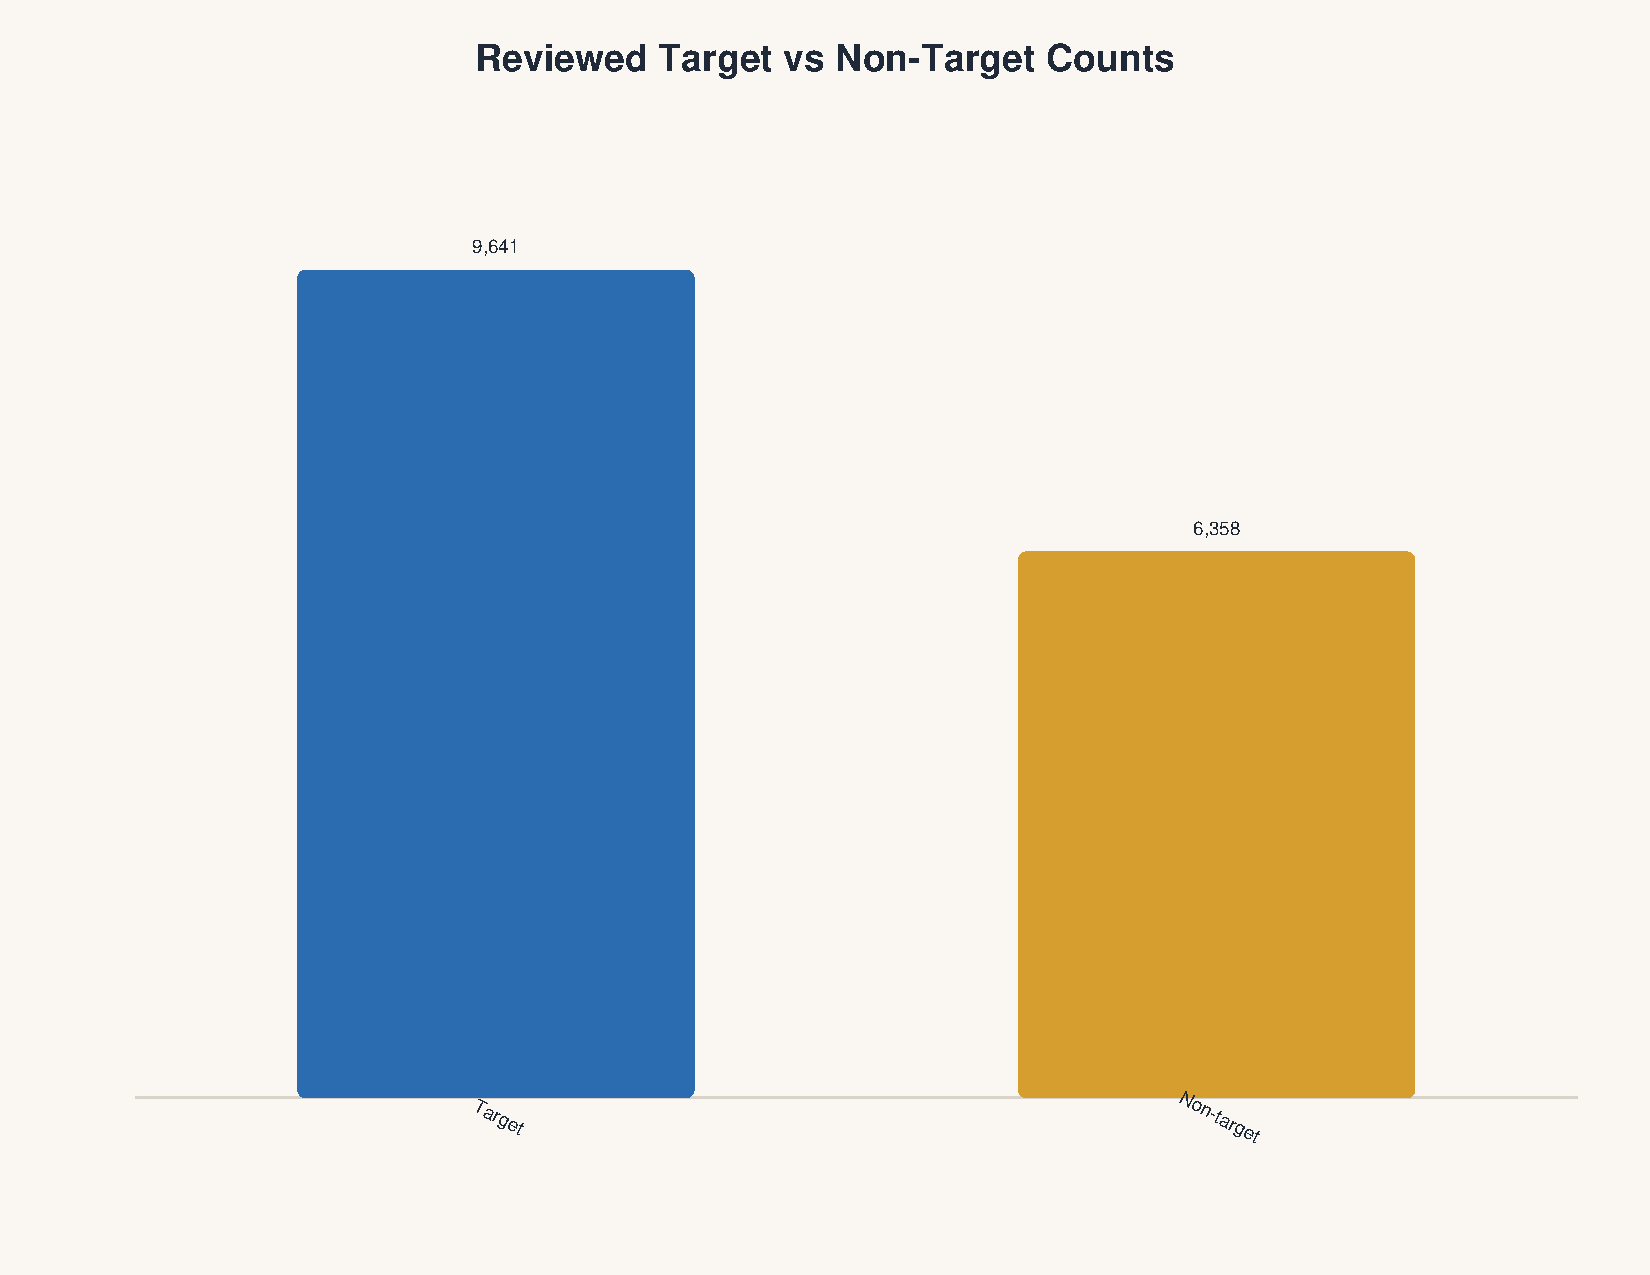
\includegraphics[width=0.75\textwidth]{../outputs/report_figures_pdf/target_vs_non_target_counts.pdf}
    \caption{Reviewed target and non-target counts in the seniority-2 modeling cohort.}
    \label{fig:targetcounts}
\end{figure}

Target-employer placement is concentrated among a small set of universities and majors. The largest target-producing schools include University of California Berkeley, University of Michigan, Cornell University, Columbia University, Duke University, University of Pennsylvania, University of Notre Dame, Northwestern University, and Vanderbilt University.

\begin{figure}[H]
    \centering
    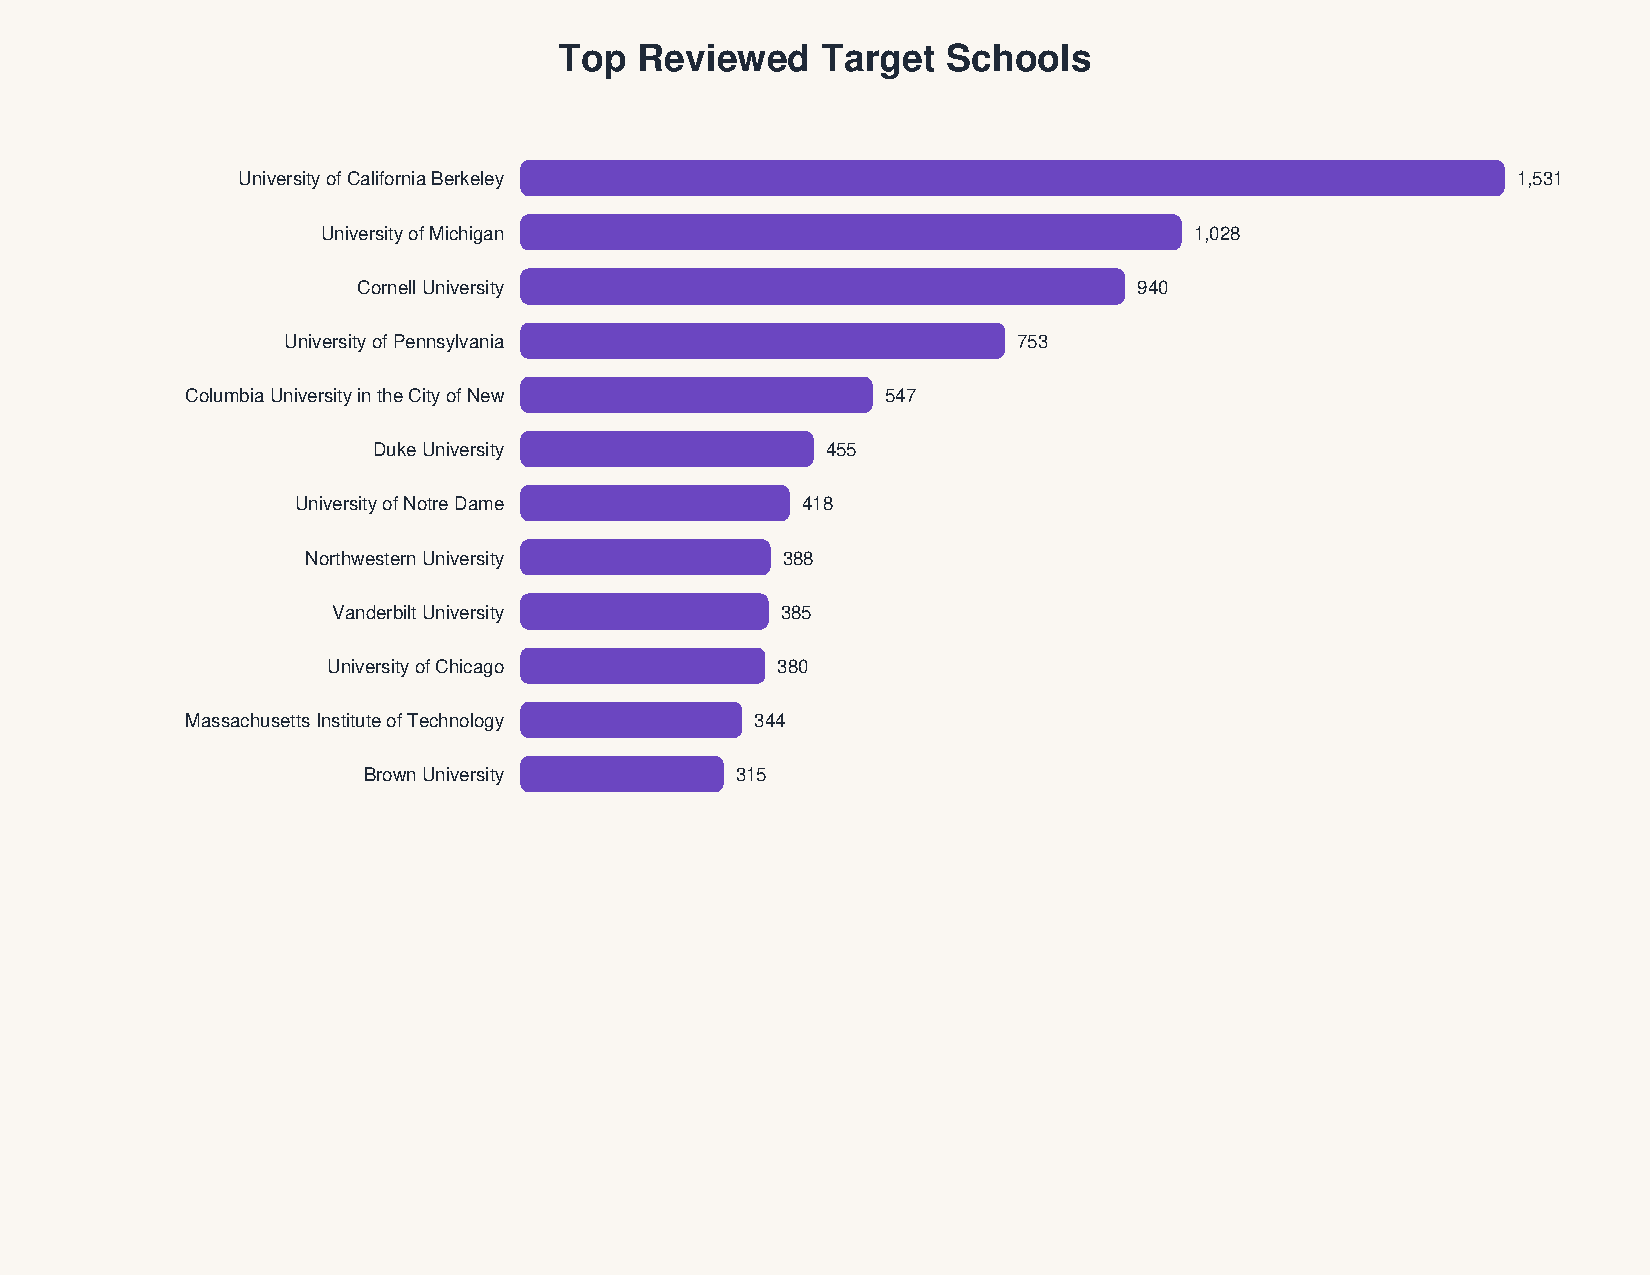
\includegraphics[width=0.85\textwidth]{../outputs/report_figures_pdf/top_target_schools.pdf}
    \caption{Top schools among users entering reviewed target employers.}
    \label{fig:topschools}
\end{figure}

We also compare the target and non-target composition within each major school. This graph answers a different question than the previous school-count plot: instead of asking which schools contribute the most target users in absolute numbers, it asks what percentage of each school's observed seniority-2 reviewed users enter a target employer.

\begin{figure}[H]
    \centering
    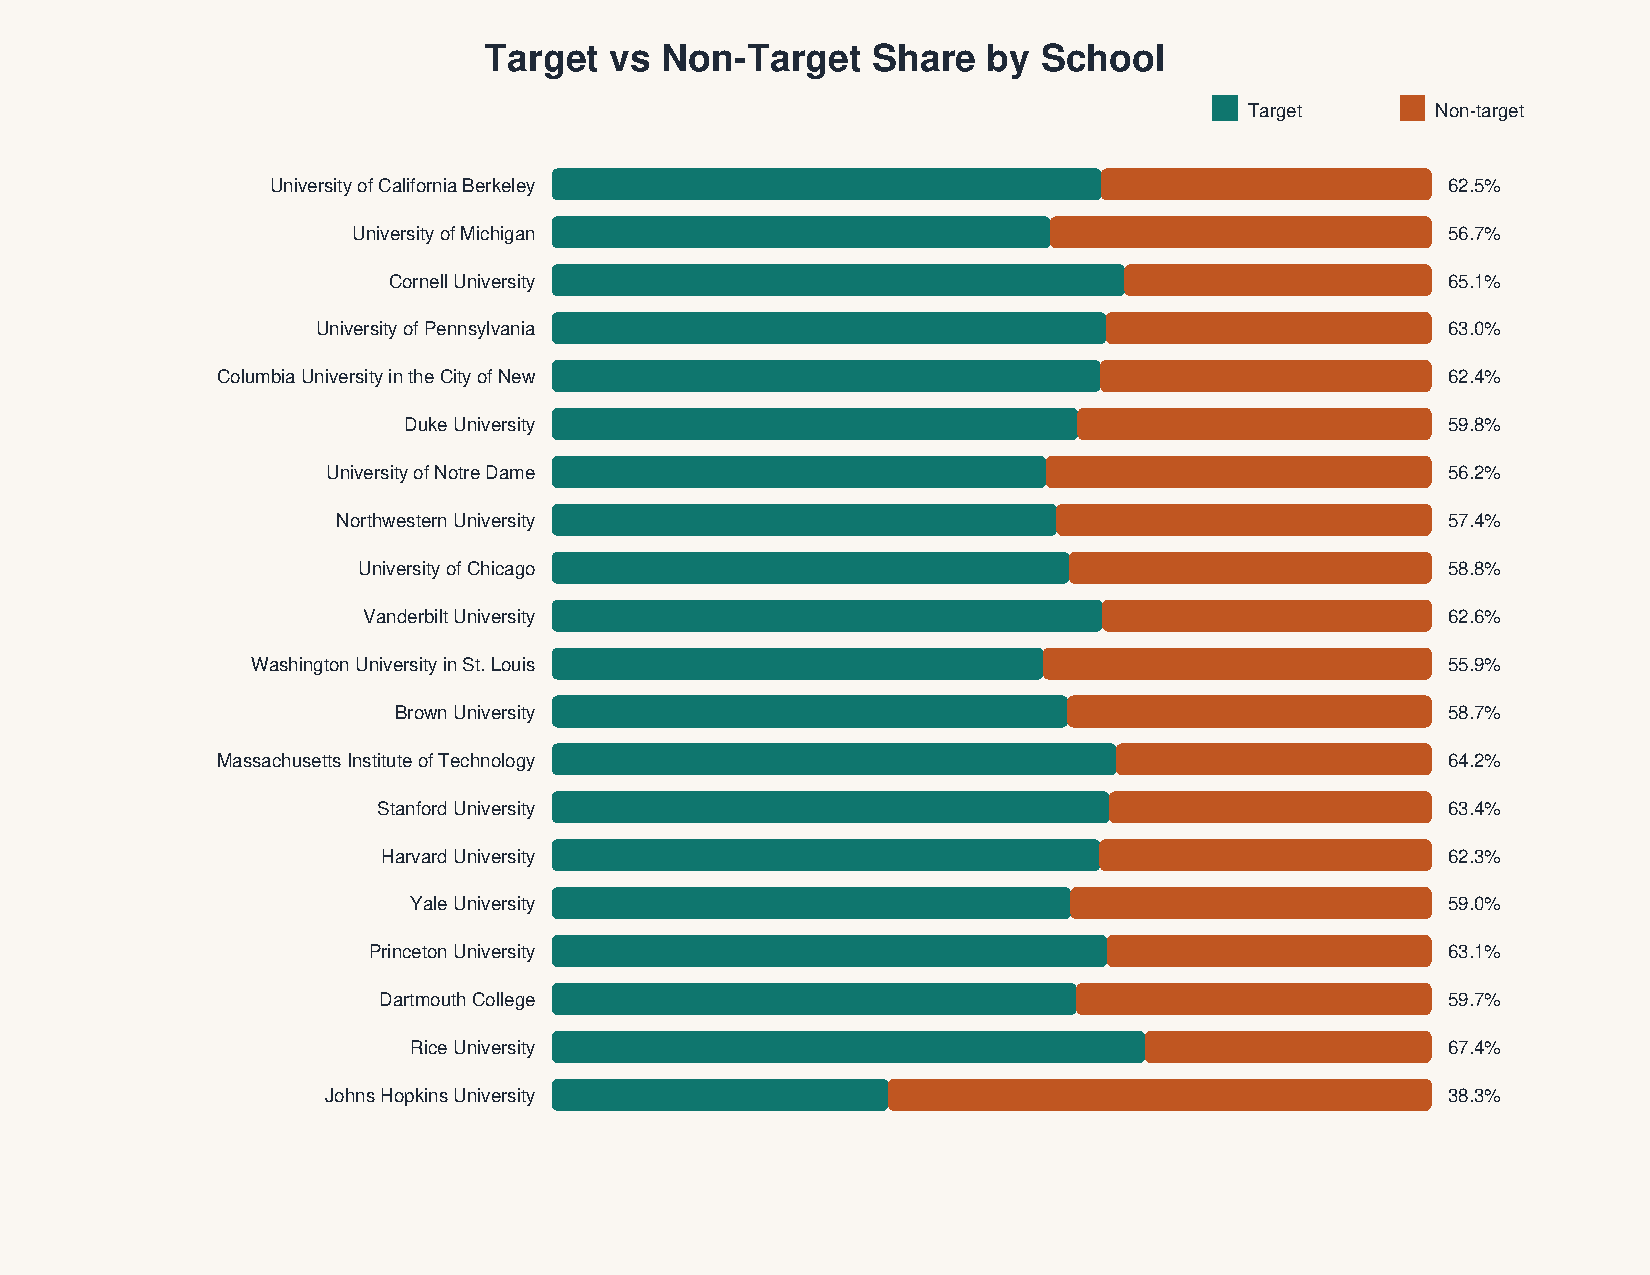
\includegraphics[width=0.9\textwidth]{../outputs/report_figures_pdf/school_target_non_target_percentages.pdf}
    \caption{Reviewed target and non-target percentages by school. Schools are shown among the largest observed school groups; Wharton is merged into University of Pennsylvania.}
    \label{fig:schoolpercent}
\end{figure}

To test whether school is associated with reviewed target-employer placement, we use a chi-square test of independence between school and target status. To avoid unstable very-small-school categories, the test is restricted to schools with at least 30 modeled users. The test includes 22 schools and 15,887 users. The chi-square statistic is 249.4 with 21 degrees of freedom, with an approximate p-value of $1.7 \times 10^{-36}$. Thus, school and target status are not independent in the observed data. The effect size, measured by Cramer's $V$, is 0.125, which suggests a statistically clear but moderate association. In other words, school matters, but it does not determine outcomes by itself.

The target-major mix is dominated by Engineering, followed by missing major, Economics, Business, Mathematics, Finance, and Statistics.

\begin{figure}[H]
    \centering
    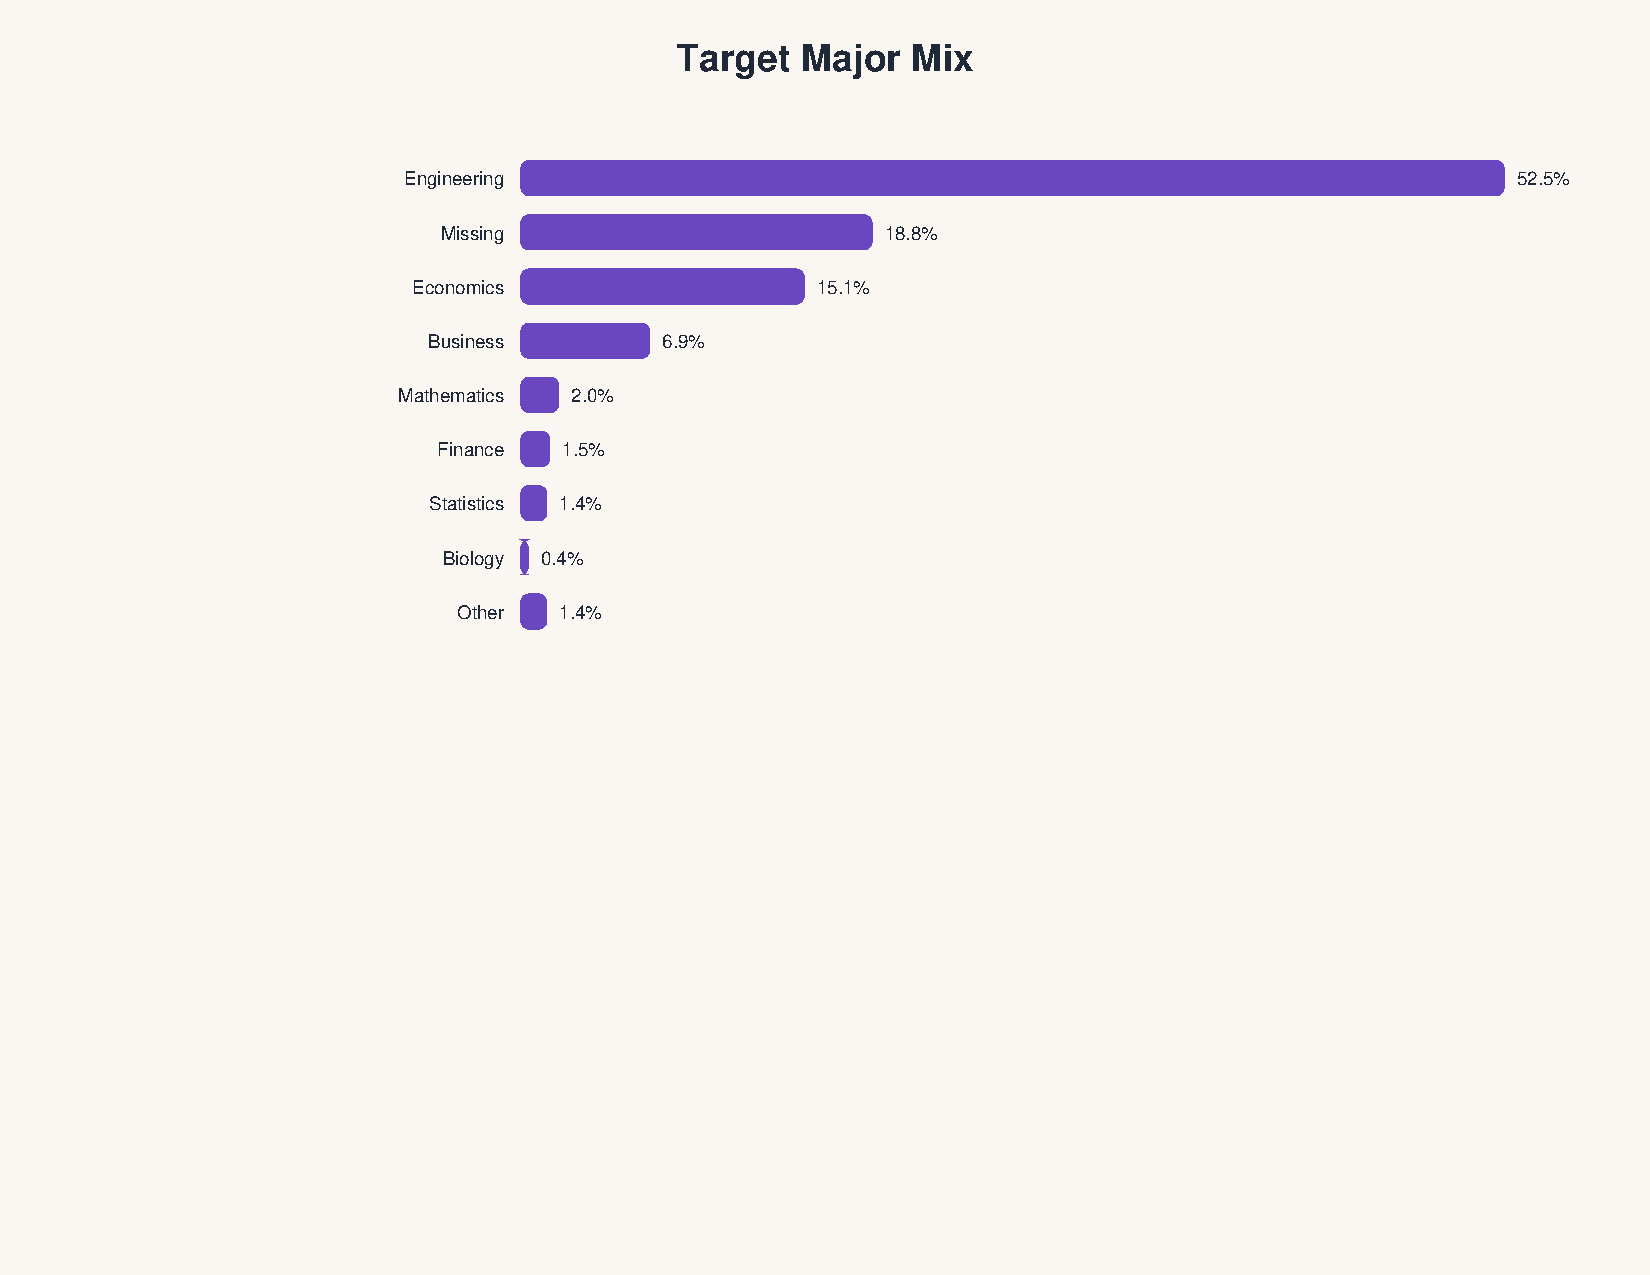
\includegraphics[width=0.85\textwidth]{../outputs/report_figures_pdf/target_major_mix.pdf}
    \caption{Major composition among reviewed target-employer users.}
    \label{fig:majormix}
\end{figure}

\section{Skill Analysis}

Skills are central to the descriptive part of this project. We aggregate user skills to the user level and compare the skill profiles of target and non-target users. Skill word clouds and frequency tables show that reviewed target outcomes are more associated with software, data, finance, business, and professional skills, while non-target outcomes are more associated with biomedical, clinical, nursing, and research-oriented skill profiles.

However, raw skill features require caution. Skills are self-reported or profile-derived, and they may be updated after a user starts work. A skill coefficient should therefore be interpreted as an association between profile content and employer pathway, not as evidence that acquiring that skill causes target-employer placement.

\subsection{Skill Differences Across 2024 and 2025}

To study the changing skill landscape, we compare skill shares among reviewed target-employer users in 2024 and 2025. Because 2025 is smaller and likely partially observed, the report emphasizes within-year percentages rather than raw counts.

Several finance, office, and professional skills have higher observed shares in 2025 among target users. Examples include Pivot Tables, Word Processing, Financial Analysis Software, Motivational Speaking, Global Project Management, Financial Data Analysis, Tax Research, and Social Media Advertising. Some software-oriented skills have lower observed shares in 2025, including Python Flask, HTML Components, Java API for RESTful Web Services, Prototype JavaScript Framework, C++, and Structured Query Language Procedural Language.

\begin{figure}[H]
    \centering
    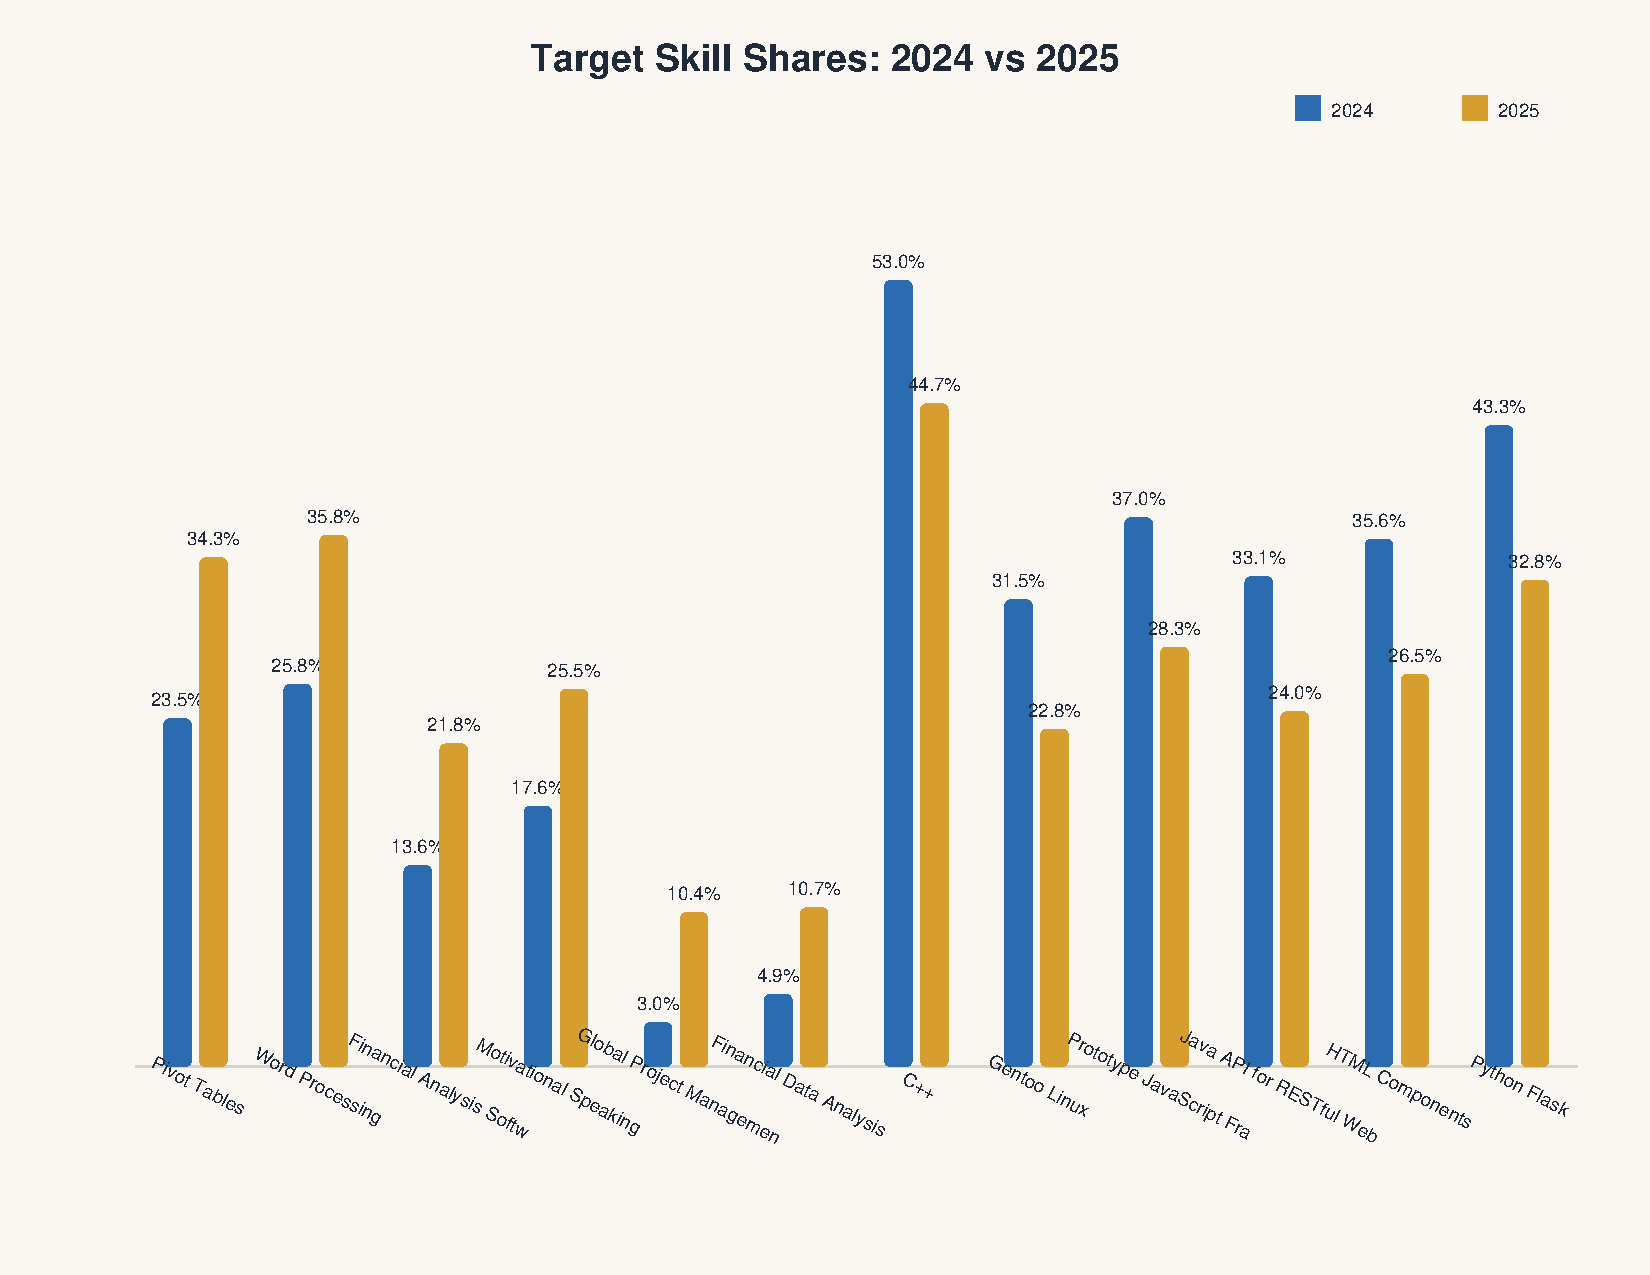
\includegraphics[width=0.9\textwidth]{../outputs/report_figures_pdf/target_skill_shares_2024_2025.pdf}
    \caption{Selected skill shares among reviewed target-employer users in 2024 and 2025. Percentages are within-year shares of observed target users.}
    \label{fig:yoyskills}
\end{figure}

These results should be interpreted as observed composition shifts, not definitive labor-market trends. The 2025 cohort is right-censored because some recent graduates may not yet have complete first-job records.

\section{PCA and K-Means Skill Profiles}

We re-ran dimensionality reduction and clustering on the cleaned seniority-2 dataset. The procedure was:

\begin{enumerate}
    \item Aggregate user skills into user-level skill sets.
    \item Select the top 250 skills by absolute smoothed log-odds comparing target and non-target users.
    \item Build a user-by-skill binary matrix.
    \item Standardize the matrix.
    \item Run singular value decomposition to obtain PCA-style components.
    \item Run k-means clustering on the first ten components.
\end{enumerate}

The first two components explain 5.5\% and 3.5\% of the variance, respectively. These shares are modest but expected for sparse skill data where many different skills each explain a small portion of variation.

\begin{figure}[H]
    \centering
    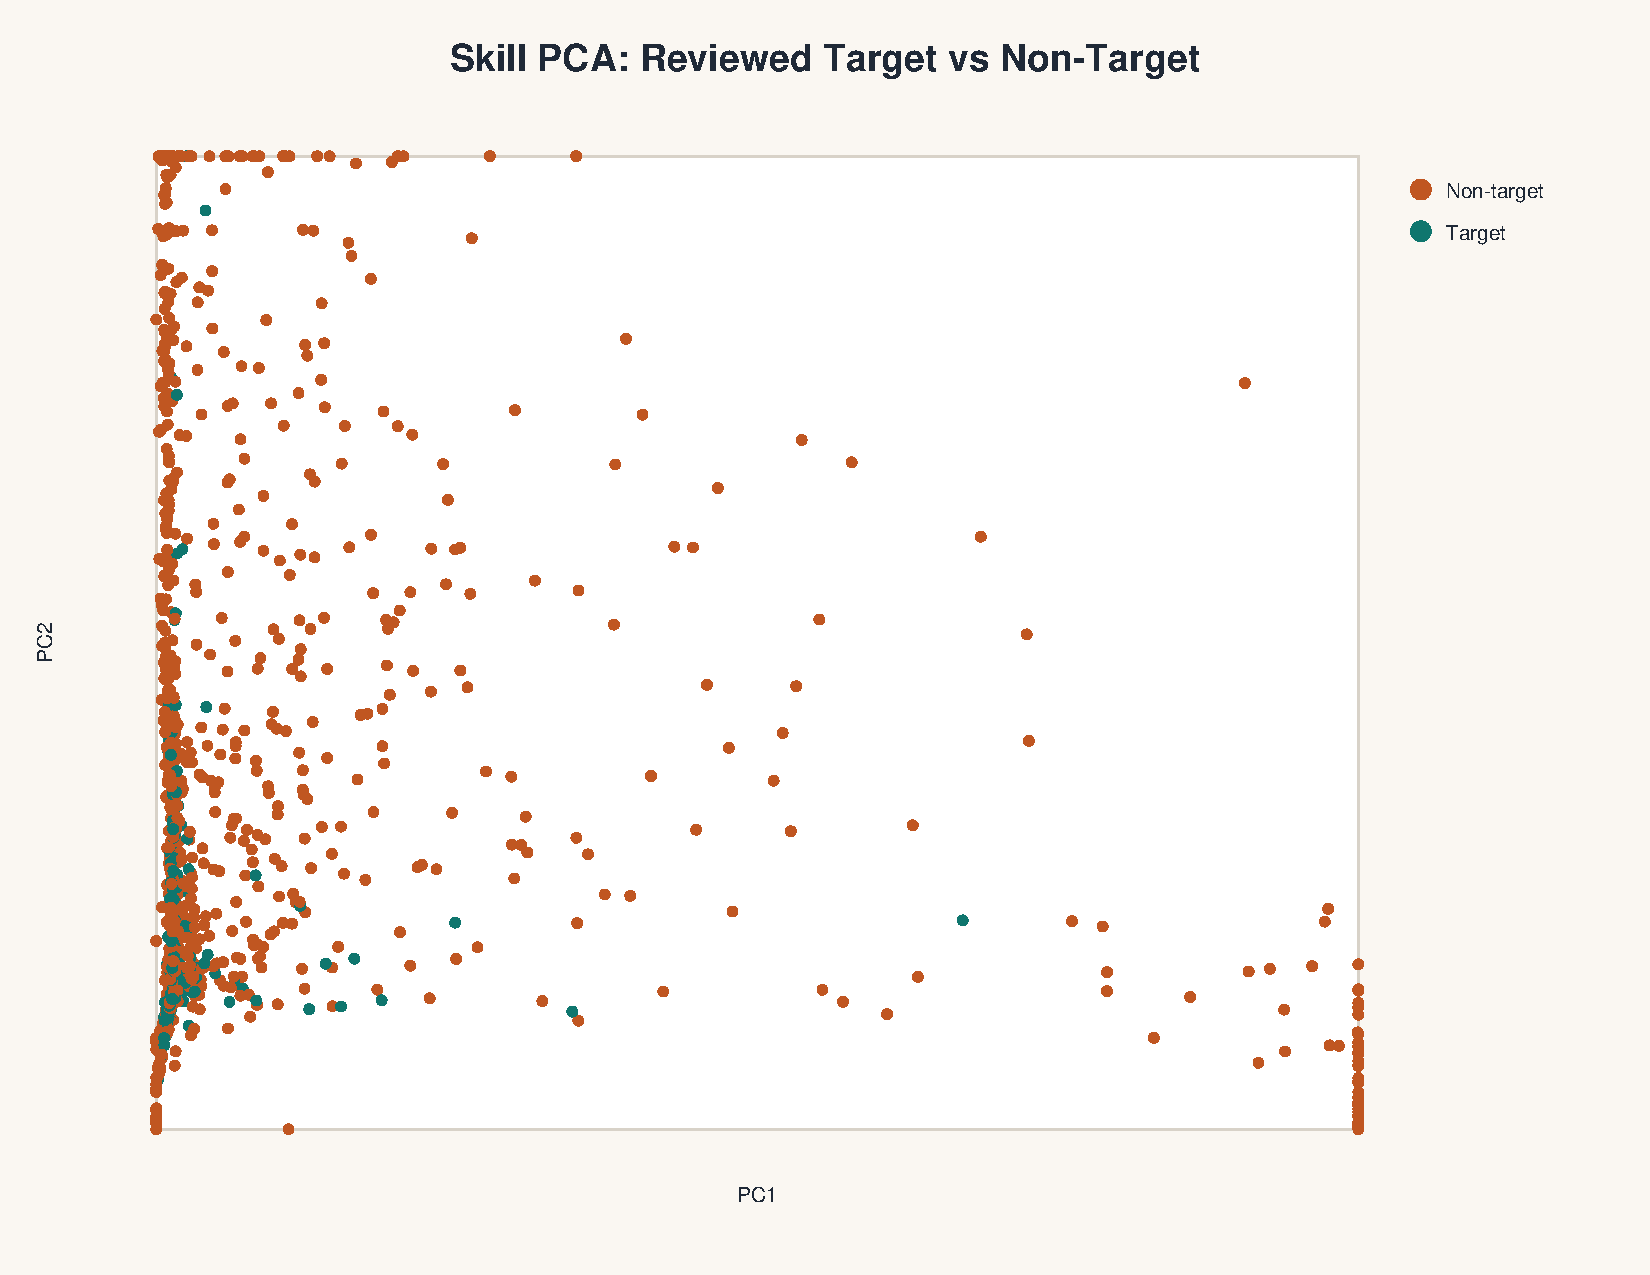
\includegraphics[width=0.8\textwidth]{../outputs/report_figures_pdf/skill_pca_target_vs_non_target.pdf}
    \caption{PCA-style skill decomposition for reviewed target and non-target users.}
    \label{fig:pca}
\end{figure}

We also use an elbow-method diagnostic to compare k-means solutions from 2 to 10 clusters. The inertia declines steadily as the number of clusters increases, with noticeable improvements through roughly six clusters. We therefore use six clusters as a descriptive compromise: enough to separate major skill-profile groups while avoiding overly fragmented clusters.

\begin{figure}[H]
    \centering
    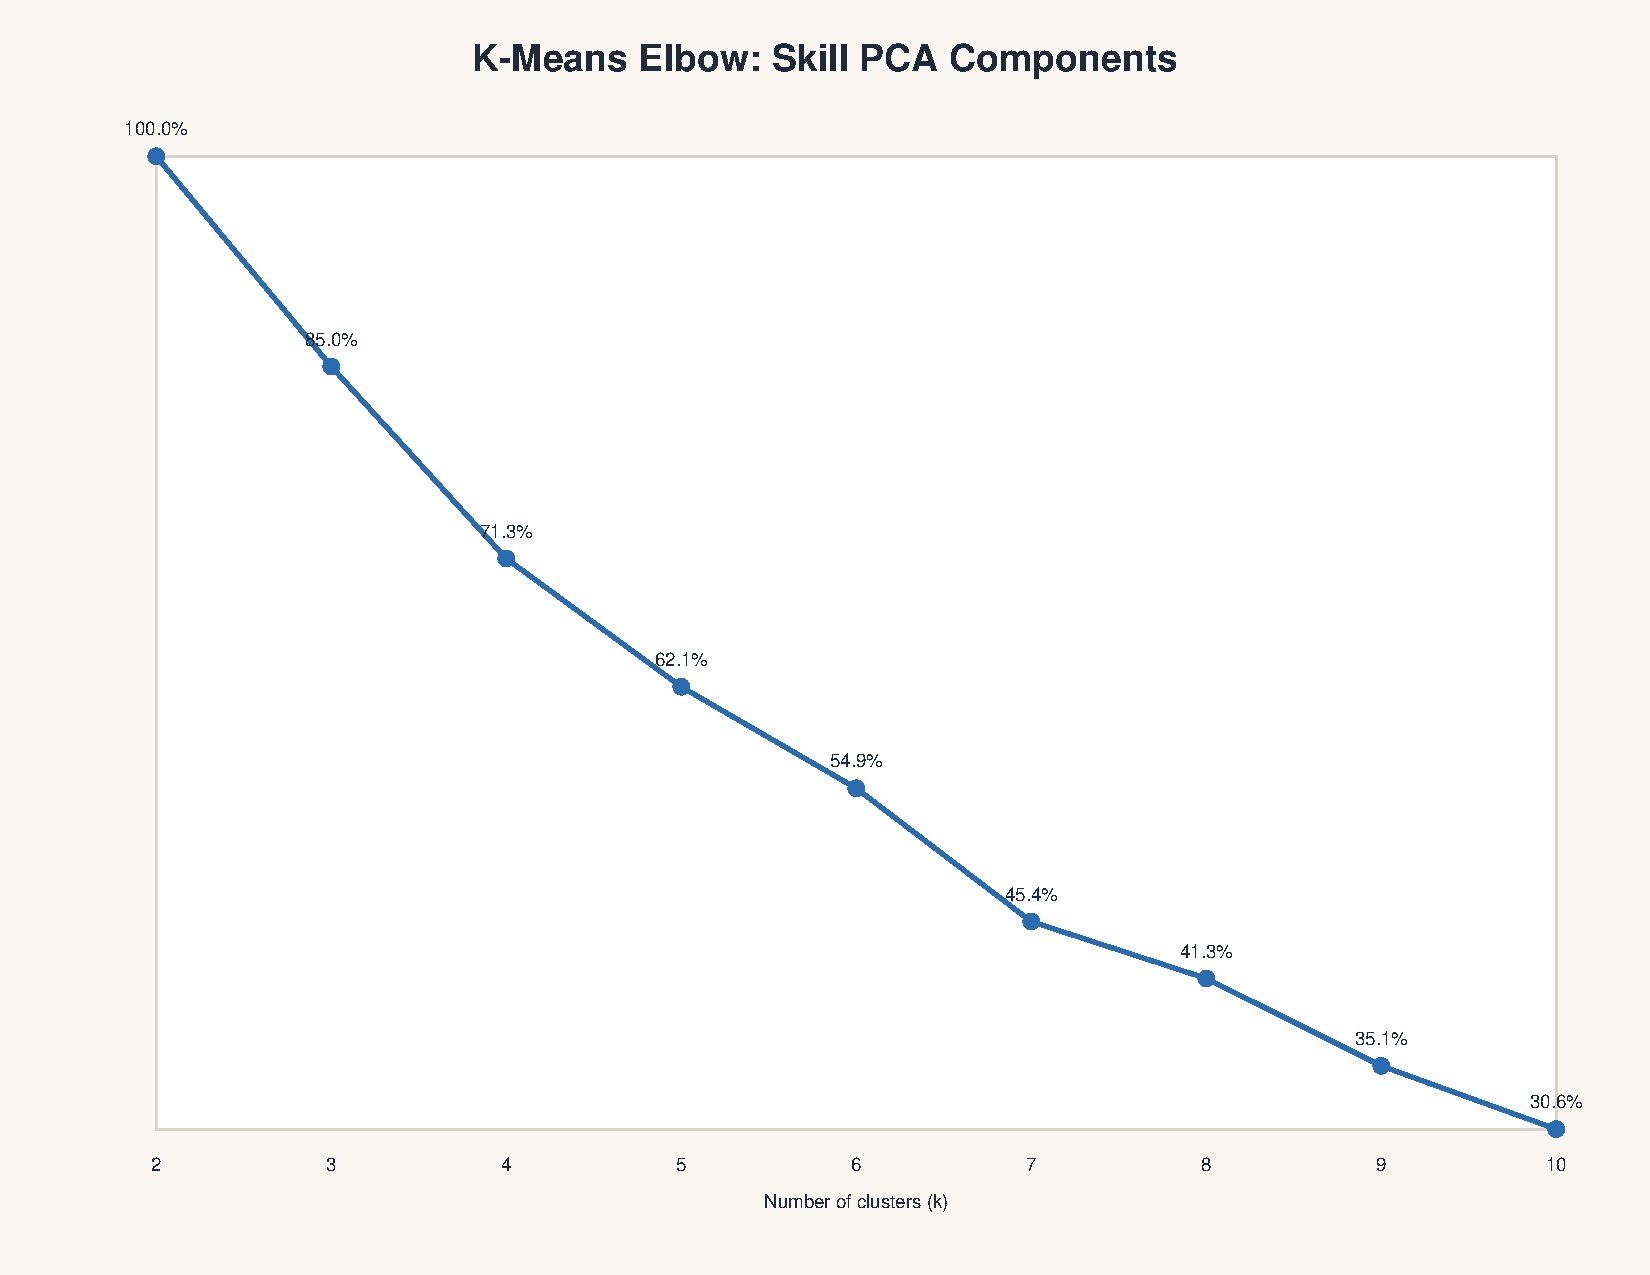
\includegraphics[width=0.75\textwidth]{../outputs/report_figures_pdf/skill_kmeans_elbow.pdf}
    \caption{Elbow-method diagnostic for k-means clustering on the first ten skill PCA components.}
    \label{fig:elbow}
\end{figure}

The k-means clusters reveal distinct skill-profile groups. The largest cluster has the highest target rate and contains broad professional, software, data, teamwork, and office-productivity skills. Smaller clusters capture legal, research/laboratory, construction/project-engineering, clinical research, and healthcare/nursing skill profiles, each with much lower target rates.

\begin{table}[H]
\centering
\caption{Skill clusters from cleaned seniority-2 PCA/k-means analysis.}
\label{tab:clusters}
\begin{tabular}{lrrrl}
\toprule
Cluster & Users & Target Users & Target Rate & Main Skill Theme \\
\midrule
4 & 14,572 & 9,593 & 65.8\% & Broad professional/software/data skills \\
1 & 149 & 9 & 6.0\% & Legal writing and litigation skills \\
2 & 718 & 32 & 4.5\% & Research, molecular biology, MATLAB \\
0 & 71 & 3 & 4.2\% & Construction/project-engineering skills \\
3 & 256 & 3 & 1.2\% & Clinical research and trial management \\
5 & 233 & 1 & 0.4\% & Healthcare, nursing, CPR, Epic EMR \\
\bottomrule
\end{tabular}
\end{table}

\begin{figure}[H]
    \centering
    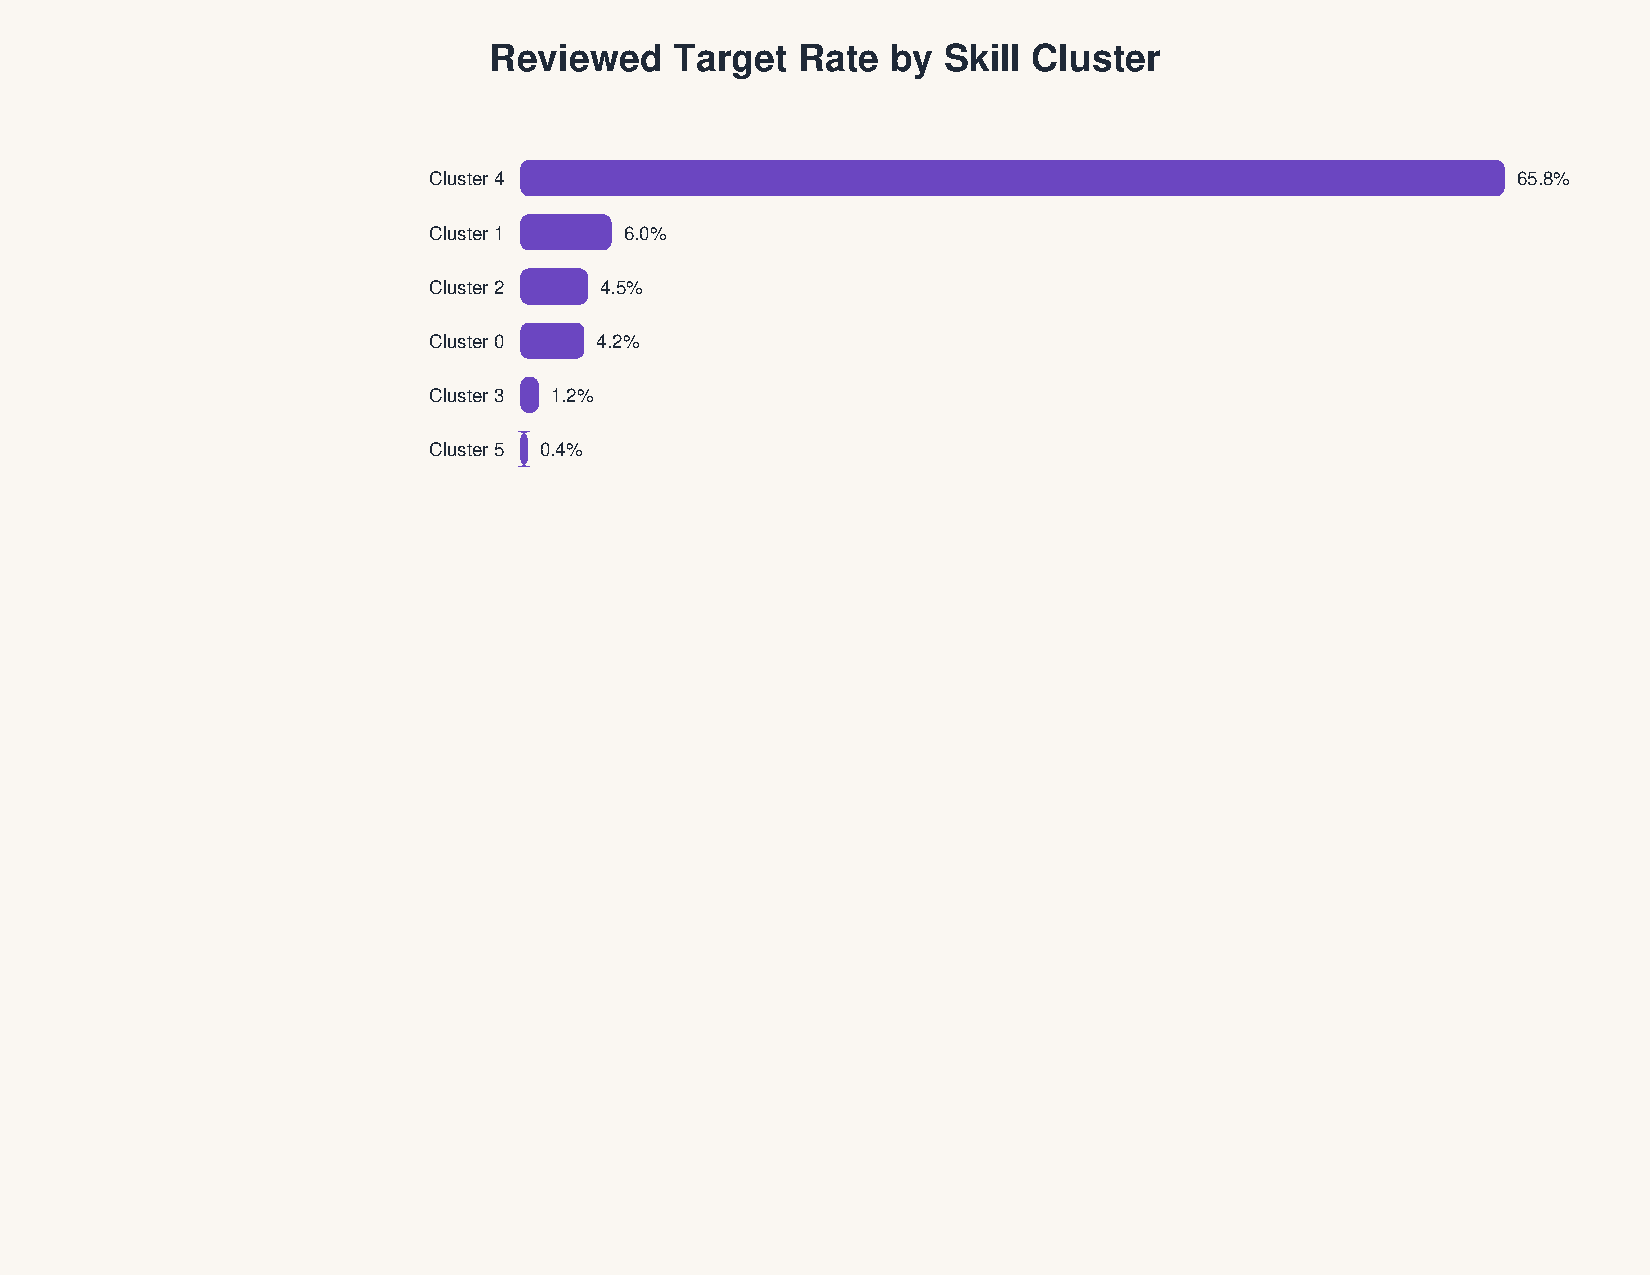
\includegraphics[width=0.75\textwidth]{../outputs/report_figures_pdf/skill_cluster_target_rates.pdf}
    \caption{Reviewed target-employer rate by skill cluster.}
    \label{fig:clusterrates}
\end{figure}

The clustering results reinforce that the reviewed target-employer label captures a specific career pathway rather than general success. Healthcare, clinical, legal, and research-heavy skill clusters may lead to valuable outcomes, but they are less represented in the target employer group used here.

\section{Prediction Models}

The project uses prediction to evaluate whether education, profile, and skill features contain signal about reviewed target-employer placement. Because the target is binary, logistic regression is both a regression model for log-odds and a classification model for predicted probabilities. In this report, we describe it as logistic classification when discussing AUC, accuracy, precision, and recall, and as logistic regression when interpreting odds ratios.

\subsection{Primary Non-Skill Logistic Classifier}

The primary interpretable model excludes raw skill indicators and \texttt{n\_skills}. This specification is intended to reduce profile-completeness and post-outcome skill-reporting bias. Features include target-encoded school, major, degree, university country, user country, prestige, number of connections, and entry-job year.

\begin{table}[H]
\centering
\caption{Primary non-skill logistic classifier performance.}
\label{tab:nonskill}
\begin{tabular}{lr}
\toprule
Metric & Test Value \\
\midrule
AUC & 0.692 \\
Accuracy & 0.678 \\
Precision & 0.699 \\
Recall & 0.819 \\
\bottomrule
\end{tabular}
\end{table}

The strongest stable predictors are major, number of connections, school, user country, and entry-job year. Major and school are target-encoded, so their coefficients indicate association with high-target-rate categories rather than causal effects.

\begin{table}[H]
\centering
\caption{Selected non-skill logistic regression coefficients.}
\label{tab:coefficients}
\begin{tabular}{lrrr}
\toprule
Feature & Log Odds & Odds Ratio & p-value \\
\midrule
Major target encoding & 0.693 & 2.000 & $<10^{-200}$ \\
Number of connections & 0.307 & 1.359 & $<10^{-50}$ \\
School target encoding & 0.251 & 1.286 & $<10^{-20}$ \\
User country target encoding & 0.113 & 1.120 & $<10^{-7}$ \\
Entry-job year & -0.099 & 0.906 & $<10^{-6}$ \\
Prestige & 0.013 & 1.013 & 0.511 \\
\bottomrule
\end{tabular}
\end{table}

\subsection{Skill-Augmented and Tree-Based Models}

We also fit exploratory skill-augmented and tree-based classifiers. The skill-augmented logistic model uses top skill indicators selected by train-only log odds. These models help answer whether skill text contains predictive signal, but they are not the cleanest models for causal or substantive interpretation.

\begin{table}[H]
\centering
\caption{Classification model comparison on the seniority-2 cohort.}
\label{tab:models}
\begin{tabular}{lrrrr}
\toprule
Model & AUC & Accuracy & Precision & Recall \\
\midrule
Skill-augmented logistic & 0.755 & 0.742 & 0.718 & 0.939 \\
Decision tree & 0.701 & 0.693 & 0.669 & 0.971 \\
Random forest & 0.732 & 0.693 & 0.666 & 0.986 \\
\bottomrule
\end{tabular}
\end{table}

\begin{figure}[H]
    \centering
    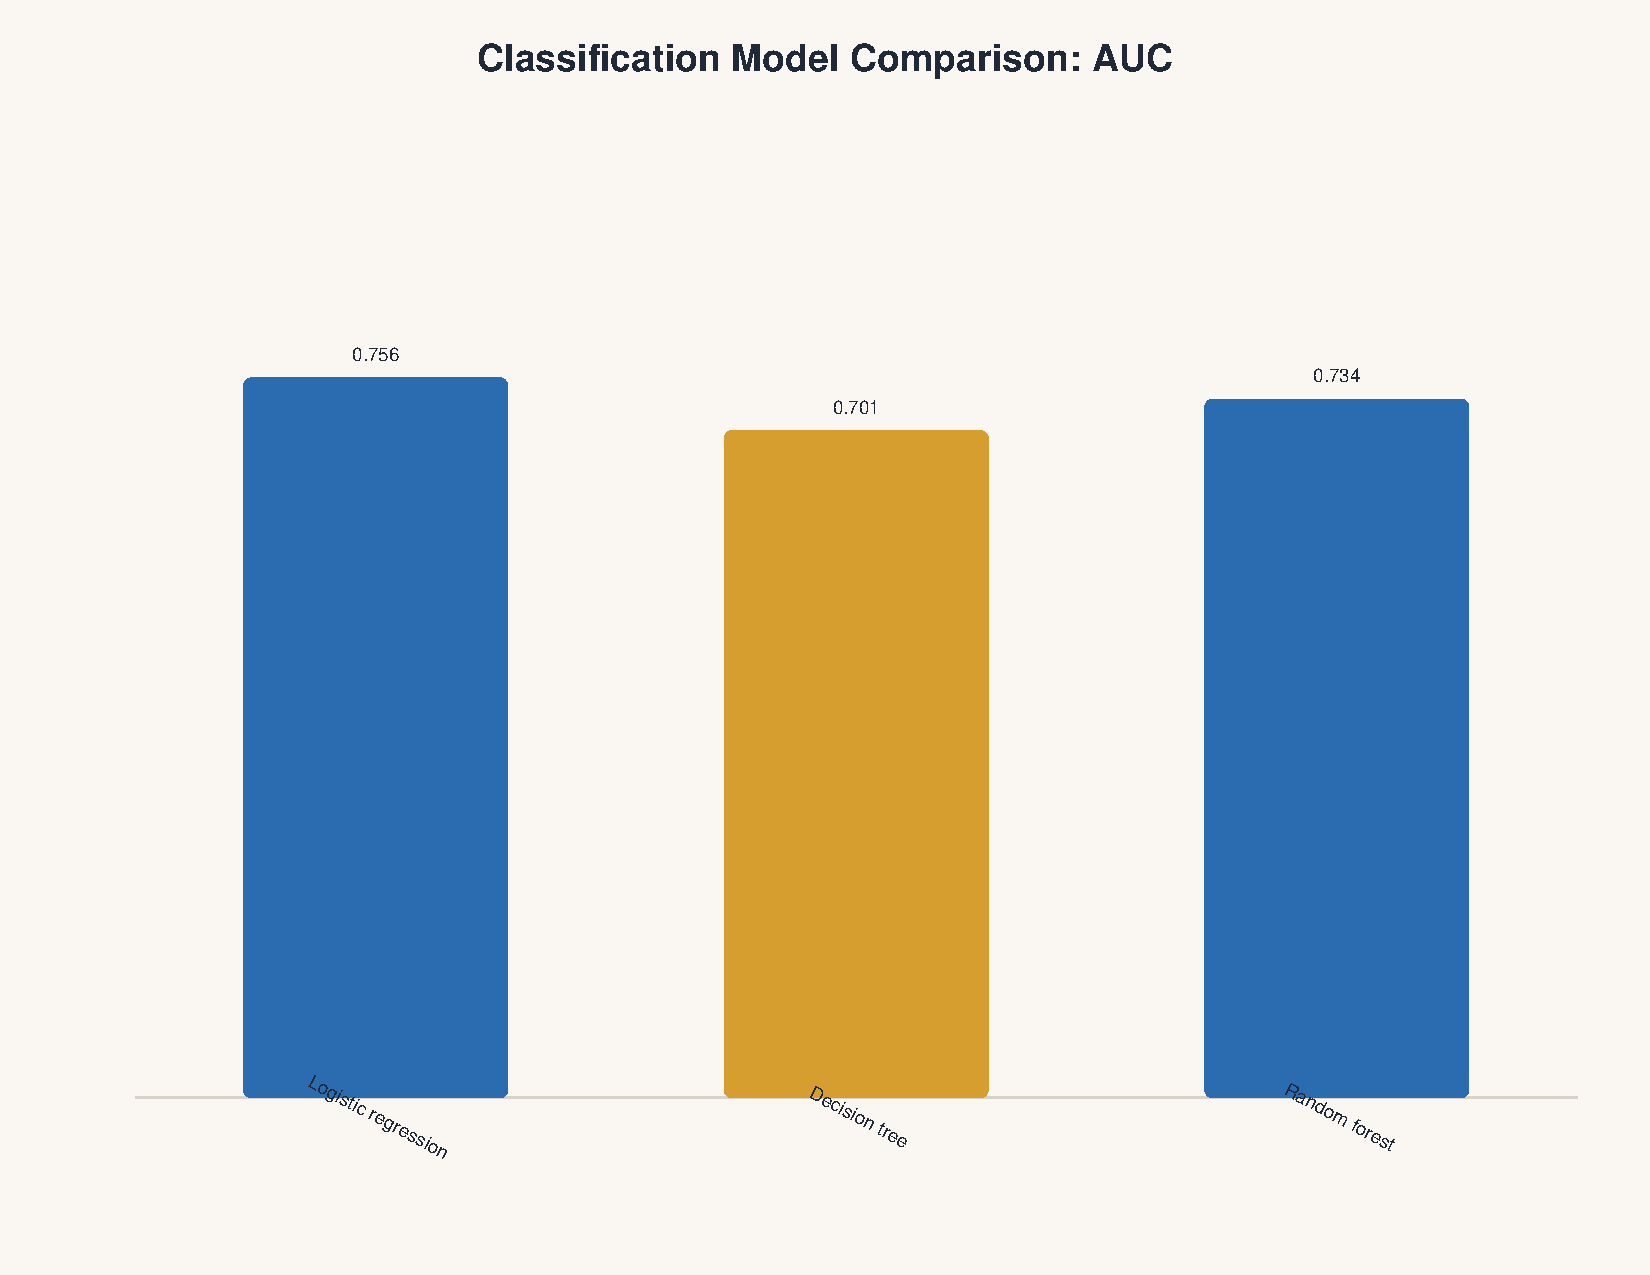
\includegraphics[width=0.72\textwidth]{../outputs/report_figures_pdf/model_comparison_auc.pdf}
    \caption{Model comparison by test AUC.}
    \label{fig:modelcomparison}
\end{figure}

The skill-augmented model improves AUC from 0.692 to 0.755, suggesting that skills contain meaningful predictive information. However, because skill data can be self-reported, incomplete, or updated after employment, the skill model should be interpreted as exploratory evidence about profile signals rather than as a causal skill-return model.

\section{2024 vs 2025 Observed Landscape}

The year-over-year section compares observed 2024 and 2025 first-job rows in the seniority-2 reviewed cohort. This is not a full time-series analysis. The 2025 sample is smaller and likely right-censored, so we use percentages to compare composition while still noting sample coverage elsewhere.

Among observed target-employer rows, the share of Software Engineering roles falls from 23.5\% in 2024 to 16.5\% in 2025. Investment Analyst falls from 8.8\% to 6.5\%. Corporate Legal rises from 0.5\% to 3.0\%, Legal Research rises from 0.3\% to 2.1\%, and Quantitative Analyst rises from 0.5\% to 1.0\%.

\begin{figure}[H]
    \centering
    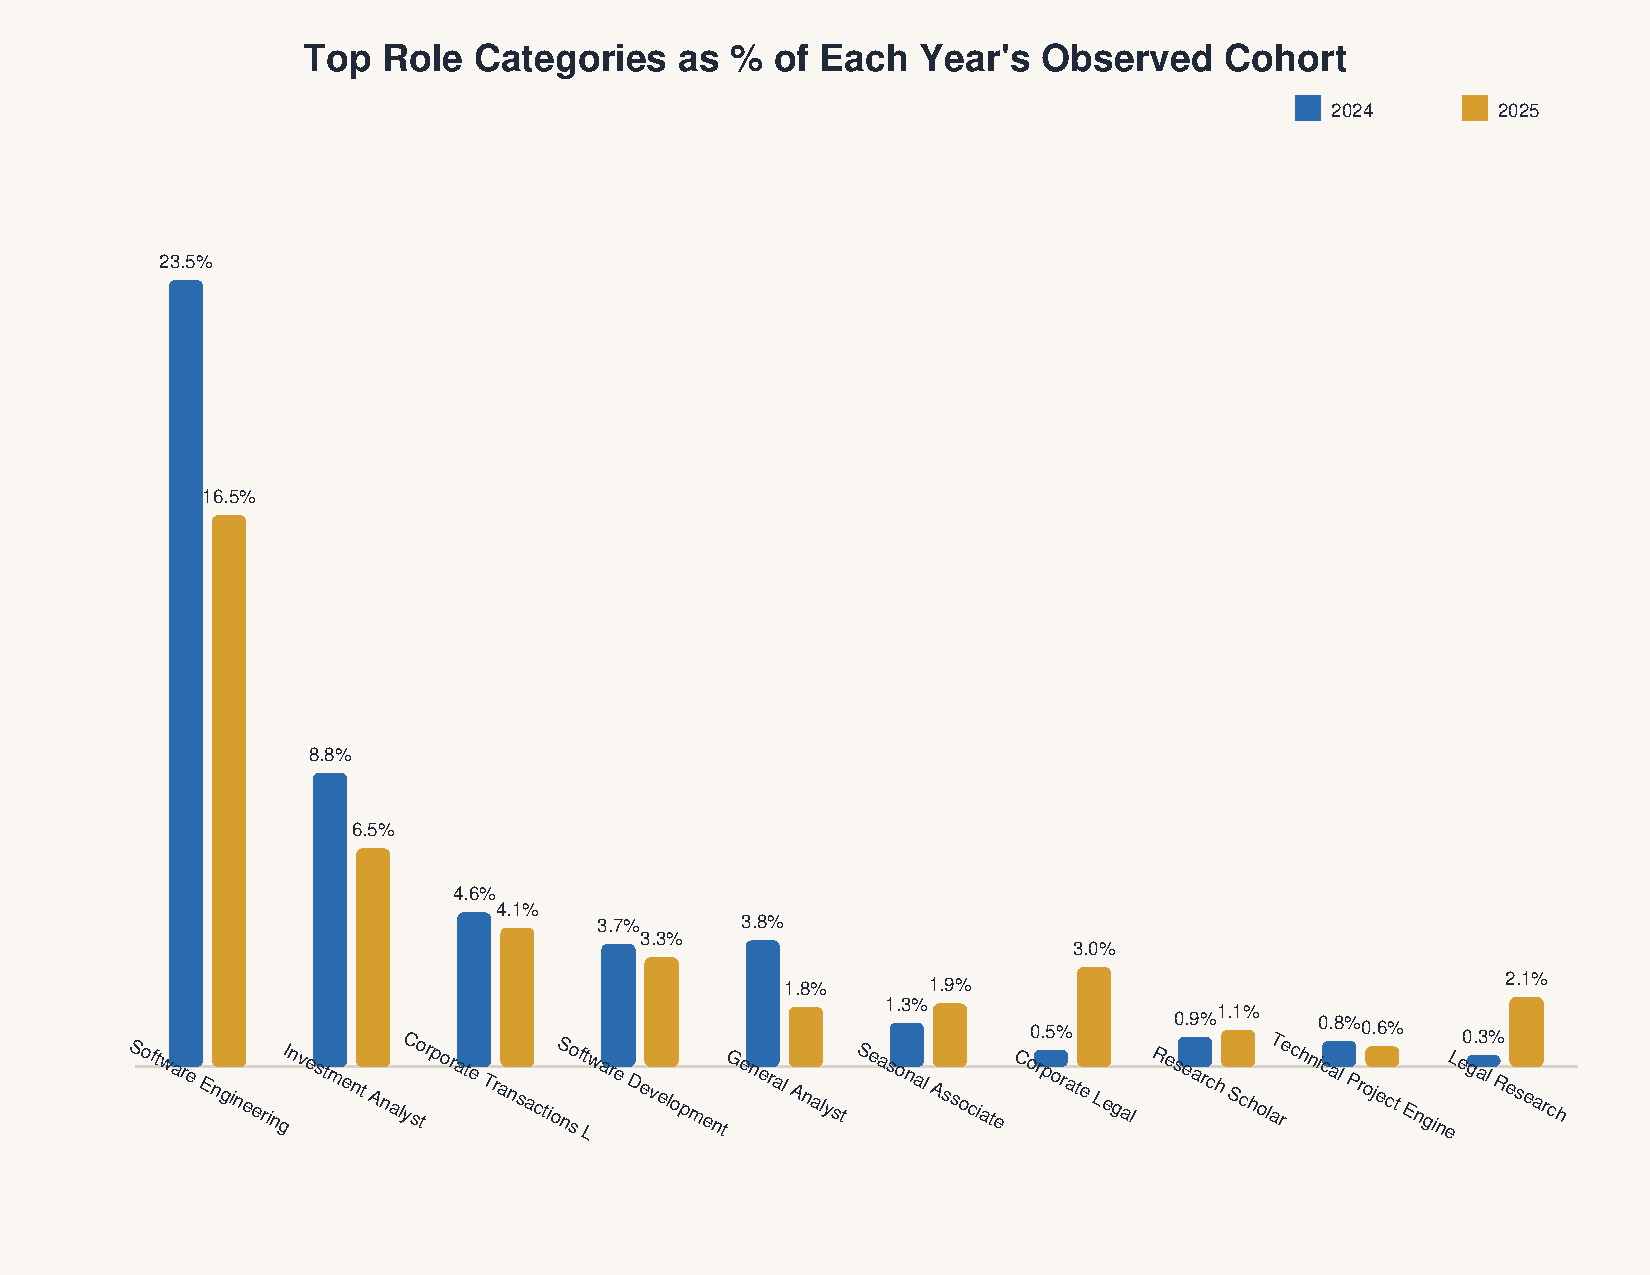
\includegraphics[width=0.9\textwidth]{../outputs/report_figures_pdf/top_role_percentages_2024_2025.pdf}
    \caption{Top role categories as percentages of each year's observed cohort. Displayed roles do not sum to 100\% because only the top categories are shown.}
    \label{fig:yoyroles}
\end{figure}

The observed skill shifts are consistent with a possible movement from software-heavy target placements toward a more mixed finance, office, and professional-services skill profile in 2025. Because of the smaller 2025 sample, this should be framed as descriptive evidence rather than a definitive labor-market trend.

\section{Discussion and Conclusion}

The cleaned analysis shows that reviewed target-employer placement is associated with both academic pathway and skill profile. The primary non-skill logistic classifier shows that major, school, connections, user country, and entry-job year are stable predictors of target placement. The skill-augmented model improves predictive performance, which supports the idea that skills contain additional signal. However, the skill signal should be interpreted carefully because skill data are self-reported/profile-derived and may be updated after employment.

The PCA and k-means analysis shows that skill profiles are not evenly distributed across employer outcomes. A broad professional/software/data cluster has the highest target rate, while healthcare, clinical research, legal, and laboratory-oriented clusters have much lower target rates. This does not imply those paths are less valuable; rather, they lead to different labor-market destinations than the reviewed target employers in this project.

The 2024-vs-2025 comparison suggests an observed decline in the share of software-engineering-heavy target roles and an increase in some finance, legal, and professional-services skill signals. Because 2025 is partially observed, this result should be presented as an observed composition shift, not a completed annual trend.

Overall, the project finds that skills matter descriptively and predictively, but the strongest reportable interpretation comes from combining skill exploration with a cautious classification pipeline and clear caveats about the reviewed-employer target definition.

\section*{Statement on AI Use}

Generative AI tools were used to assist with code development, debugging, report organization, figure generation, and interpretation of model outputs. The group reviewed and edited the outputs to ensure that the final analysis, interpretations, and conclusions matched the project data and objectives.

\appendix

\section{Appendix: Reproducible Pipeline}

The main reproducible script is:

\begin{verbatim}
scripts/run_ready_analysis_classification.py
\end{verbatim}

The LaTeX-friendly PDF figures were generated with:

\begin{verbatim}
scripts/create_latex_report_assets.py
\end{verbatim}

Important output files include:

\begin{itemize}
    \item \texttt{outputs/tables/final/ready\_analysis\_results\_summary\_report.md}
    \item \texttt{outputs/tables/final/ready\_classification\_report.md}
    \item \texttt{outputs/tables/final/ready\_non\_skill\_logistic\_metrics.csv}
    \item \texttt{outputs/tables/final/ready\_skill\_cluster\_profiles.csv}
    \item \texttt{outputs/tables/final/ready\_yoy\_2024\_2025\_target\_skill\_shift.csv}
\end{itemize}

\section{Appendix: Key Limitations}

The analysis is observational and cannot establish causality. Employer labels apply only to reviewed employers, and unreviewed employers are excluded from supervised modeling. The \texttt{seniority == 2} filter improves scope clarity but narrows generalizability. Skills are self-reported/profile-derived and may not represent pre-employment ability. The 2025 comparison is partially observed and should not be interpreted as a complete labor-market trend.

\end{document}
